\documentclass[xetex,mathserif,serif]{beamer}
\usepackage{polyglossia}
\setdefaultlanguage[babelshorthands=true]{russian}
\usepackage{minted}

\useoutertheme{infolines}

\setmainfont{FreeSans}
\newfontfamily{\russianfonttt}{FreeSans}

\title{Принципы SOLID}
\author[Юрий Литвинов]{Юрий Литвинов \newline \textcolor{gray}{\small\texttt{yurii.litvinov@gmail.com}}}
\date{20.10.2017г}

\begin{document}
	
	\frame{\titlepage}

	\section{Принципы SOLID}

	\begin{frame}
		\frametitle{Принципы SOLID}
		\begin{itemize}
			\item Single responsibility principle
			\item Open/closed principle
			\item Liskov substitution principle
			\item Interface segregation principle
			\item Dependency inversion principle
		\end{itemize}
	\end{frame}

	\begin{frame}
		\frametitle{Single responsibility principle}
		\begin{itemize}
			\item Каждый объект должен иметь одну обязанность
			\item Эта обязанность должна быть полностью инкапсулирована в класс
		\end{itemize}
		\begin{flushright}
			
\includegraphics[width=0.25\textwidth]{singleResponsibility.png}
		\end{flushright}
	\end{frame}

	\begin{frame}
		\frametitle{Open/closed principle}
		\begin{itemize}
			\item программные сущности (классы, модули, функции и т. п.) должны быть открыты для расширения, но закрыты для изменения
			\begin{itemize}
				\item переиспользование через наследование
				\item неизменные интерфейсы
			\end{itemize}
		\end{itemize}
		\begin{flushright}
			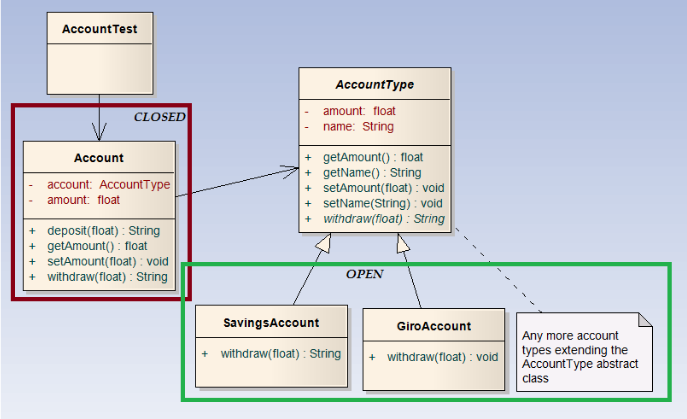
\includegraphics[width=0.5\textwidth]{openClosedPrinciple.png}
		\end{flushright}
	\end{frame}

	\begin{frame}
		\frametitle{Liskov substitution principle}
		\begin{itemize}
			\item Функции, которые используют базовый тип, должны иметь возможность использовать подтипы базового типа, не зная об этом
		\end{itemize}
		\begin{flushright}
			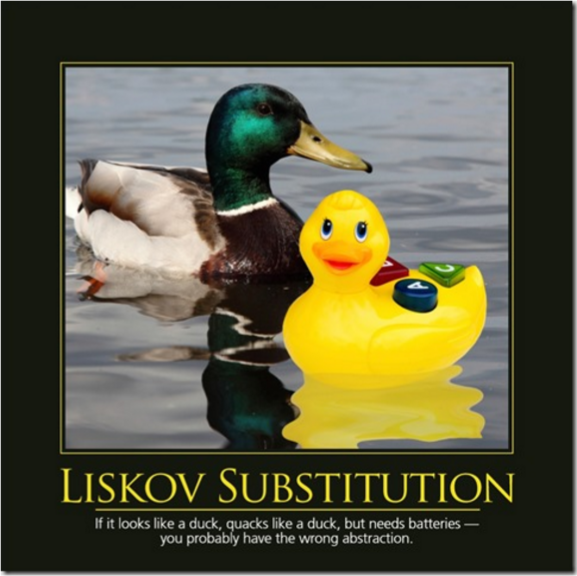
\includegraphics[width=0.4\textwidth]{liskovSubstitutionPrinciple.png}
		\end{flushright}
	\end{frame}

	\begin{frame}
		\frametitle{Interface segregation principle}
		\begin{itemize}
			\item Клиенты не должны зависеть от методов, которые они не используют
			\begin{itemize}
				\item слишком ``толстые'' интерфейсы необходимо разделять на более мелкие и специфические
			\end{itemize}
		\end{itemize}
		\begin{flushright}
			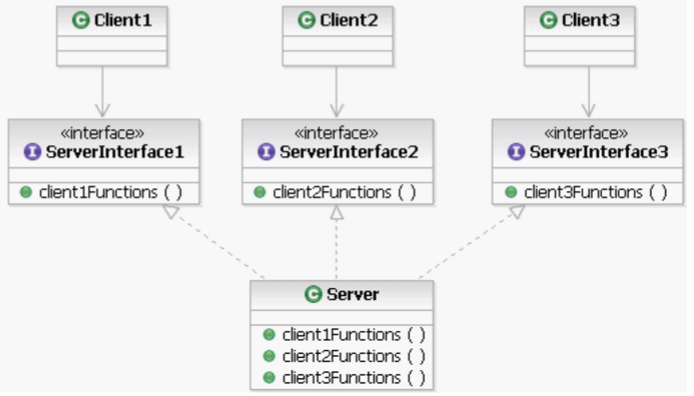
\includegraphics[width=0.5\textwidth]{interfaceSegregationPrinciple.png}
		\end{flushright}
	\end{frame}

	\begin{frame}
		\frametitle{Dependency inversion principle}
		\begin{itemize}
			\item Модули верхних уровней не должны зависеть от модулей нижних уровней. Оба типа модулей должны зависеть от абстракций
			\item Абстракции не должны зависеть от деталей. Детали должны зависеть от абстракций
		\end{itemize}
		\begin{flushright}
			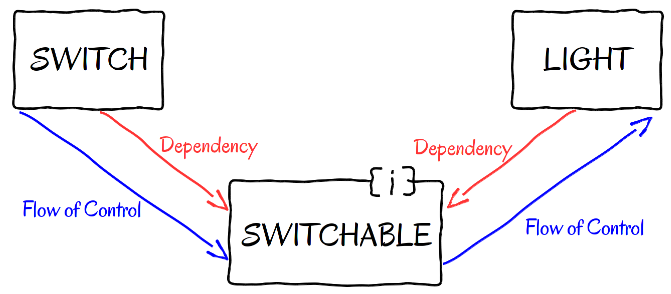
\includegraphics[width=0.5\textwidth]{dependencyInversionPrinciple.png}
		\end{flushright}
	\end{frame}

	\begin{frame}
		\frametitle{Закон Деметры}
		\begin{itemize}
			\item ``Не разговаривай с незнакомцами!''
			\item Объект A не должен иметь возможность получить непосредственный доступ к объекту C, если у объекта A есть доступ к объекту B, и у объекта B есть доступ к объекту C
			\begin{itemize}
				\item \mintinline{java}|book.pages.last.text|
				\item \mintinline{java}|book.pages().last().text()|
				\item \mintinline{java}|book.lastPageText()|
			\end{itemize}
		\end{itemize}
	\end{frame}

	\section{Технические подробности}

	\begin{frame}
		\frametitle{Абстрактные типы данных}
		\begin{itemize}
			\item \mintinline{java}|currentFont.size = 16| --- плохо
			\item \mintinline{java}|currentFont.size = PointsToPixels(12)| --- чуть лучше
			\item \mintinline{java}|currentFont.sizeInPixels = PointsToPixels(12)| --- ещё чуть лучше
			\item \mintinline{java}|currentFont.setSizeInPoints(sizeInPoints)| \newline
					\mintinline{java}|currentFont.setSizeInPixels(sizeInPixels)| --- совсем хорошо
		\end{itemize}
	\end{frame}

	\begin{frame}[fragile]
		\frametitle{Пример плохой абстракции}
		\begin{minted}{java}
public class Program {
   public void initializeCommandStack() { ... }
   public void pushCommand(Command command) { ... }
   public Command popCommand() { ... }
   public void shutdownCommandStack() { ... }
   public void initializeReportFormatting() { ... }
   public void formatReport(Report report) { ... }
   public void printReport(Report report) { ... }
   public void initializeGlobalData() { ... }
   public void shutdownGlobalData() { ... }
}
		\end{minted}
\end{frame}

	\begin{frame}[fragile]
		\frametitle{Пример хорошей абстракции}
		\begin{footnotesize}
			\begin{minted}{java}
public class Employee {
   public Employee(
           FullName name,
           String address,
           String workPhone,
           String homePhone,
           TaxId taxIdNumber,
           JobClassification jobClass
   ) { ... }

   public FullName getName() { ... }
   public String getAddress() { ... }
   public String getWorkPhone() { ... }
   public String getHomePhone() { ... }
   public TaxId getTaxIdNumber() { ... }
   public JobClassification getJobClassification() { ... }
}
			\end{minted}
		\end{footnotesize}
\end{frame}

	\begin{frame}[fragile]
		\frametitle{Уровень абстракции (плохо)}
		\begin{minted}{java}
public class EmployeeRoster implements MyList<Employee> {
   public void addEmployee(Employee employee) { ... }
   public void removeEmployee(Employee employee) { ... }
   public Employee nextItemInList() { ... }
   public Employee firstItem() { ... }
   public Employee lastItem() { ... }
}
		\end{minted}
\end{frame}

	\begin{frame}[fragile]
		\frametitle{Уровень абстракции (хорошо)}
		\begin{minted}{java}
public class EmployeeRoster {
   public void addEmployee(Employee employee) { ... }
   public void removeEmployee(Employee employee) { ... }
   public Employee nextEmployee() { ... }
   public Employee firstEmployee() { ... }
   public Employee lastEmployee() { ... }
}
		\end{minted}
\end{frame}

	\begin{frame}
		\frametitle{Общие рекомендации}
		\begin{itemize}
			\item Про каждый класс знайте, реализацией какой абстракции он является
			\item Учитывайте противоположные методы (add/remove, on/off, ...)
			\item Соблюдайте принцип единственности ответственности
			\begin{itemize}
				\item Может потребоваться разделить класс на несколько разных классов просто потому, что методы по смыслу слабо связаны
			\end{itemize}
			\item По возможности делайте некорректные состояния невыразимыми в системе типов
			\begin{itemize}
				\item Комментарии в духе ``не пользуйтесь объектом, не вызвав  init()'' можно заменить конструктором
			\end{itemize}
			\item При рефакторинге надо следить, чтобы интерфейсы не деградировали
		\end{itemize}
	\end{frame}

	\begin{frame}[fragile]
		\frametitle{Инкапсуляция}
		\begin{itemize}
			\item Принцип минимизации доступности методов
			\item Паблик-полей не бывает:
		\end{itemize}
		\begin{columns}
			\begin{column}{0.25\textwidth}
				\begin{minted}{java}
class Point {
   public float x;
   public float y;
   public float z;
}
				\end{minted}
			\end{column}
			\begin{column}{0.1\textwidth}
				vs
			\end{column}
			\begin{column}{0.5\textwidth}
				\begin{minted}{java}
class Point {
   private float x;
   private float y;
   private float z;
   public float getX() { ... }
   public float getY() { ... }
   public float getZ() { ... }
   public void setX(float x) { ... }
   public void setY(float y) { ... }
   public void setZ(float z) { ... }
}
				\end{minted}
			\end{column}
		\end{columns}
\end{frame}

	\begin{frame}
		\frametitle{Ещё рекомендации}
		\begin{itemize}
			\item Класс не должен ничего знать о своих клиентах
			\item Лёгкость чтения кода важнее, чем удобство его написания
			\item Опасайтесь семантических нарушений инкапсуляции
			\begin{itemize}
				\item ``Не будем вызывать ConnectToDB(), потому что GetRow() сам его вызовет, если соединение не установлено'' --- это программирование \textit{сквозь} интерфейс
			\end{itemize}
			\item Protected- и package- полей тоже не бывает
			\begin{itemize}
				\item На самом деле, у класса два интерфейса --- для внешних объектов и для потомков (может быть отдельно третий, для классов внутри пакета, но это может быть плохо)
			\end{itemize}
		\end{itemize}
	\end{frame}

	\begin{frame}
		\frametitle{Наследование}
		\begin{itemize}
			\item Включение лучше
			\begin{itemize}
				\item Переконфигурируемо во время выполнения
				\item Более гибко
				\item Иногда более естественно
			\end{itemize}
			\item Наследование --- отношение ``является'', закрытого наследования не бывает
			\begin{itemize}
				\item Наследование --- это наследование интерфейса (полиморфизм подтипов, subtyping)
			\end{itemize}
			\item Хороший тон --- явно запрещать наследование (final- или sealed-классы)
			\item Не вводите новых методов с такими же именами, как у родителя
			\item Code smells:
			\begin{itemize}
				\item Базовый класс, у которого только один потомок
				\item Пустые переопределения
				\item Очень много уровней в иерархии наследования
			\end{itemize}
		\end{itemize}
	\end{frame}

	\begin{frame}[fragile]
		\frametitle{Пример}
		\begin{footnotesize}
			\begin{columns}
				\begin{column}{0.35\textwidth}
					\begin{minted}{java}
class Operation {
   private char sign = '+';
   private int left;
   private int right;
   public int eval()
   {
       switch (sign) {
           case '+': return left + right;
       }
       throw new RuntimeException();
   }
}
					\end{minted}
				\end{column}
				\begin{column}{0.1\textwidth}
					vs
				\end{column}
				\begin{column}{0.45\textwidth}
					\begin{minted}{java}
abstract class Operation {
   private int left;
   private int right;
   protected int getLeft() { return left; }
   protected int getRight() { return right; }
   abstract public int eval();
}

class Plus extends Operation {
   @Override public int eval() { 
        return getLeft() + getRight(); 
   }
}
					\end{minted}
				\end{column}
			\end{columns}
		\end{footnotesize}
\end{frame}

	\begin{frame}
		\frametitle{Конструкторы}
		\begin{itemize}
			\item Инициализируйте все поля, которые надо инициализировать
			\begin{itemize}
				\item После конструктора должны выполняться все инварианты
			\end{itemize}
			\item НЕ вызывайте виртуальные методы из конструктора
			\item private-конструкторы для объектов, которые не должны быть созданы (или одиночек)
			\item Deep copy предпочтительнее Shallow copy
			\begin{itemize}
				\item Хотя второе может быть эффективнее
			\end{itemize}
		\end{itemize}
	\end{frame}

	\begin{frame}
		\frametitle{Когда создавать классы}
		\begin{itemize}
			\item Объекты предметной области
			\item Абстрактные объекты
			\item Изоляция сложности
			\item Сокрытие деталей реализации
			\item Изоляция изменчивости
			\item Упаковка родственных операций
			\begin{itemize}
				\item Статические классы вполне ок
			\end{itemize}
		\end{itemize}
	\end{frame}

\end{document}